\section{Our publications}

\subsection{Geography}

\paragraph{Maximising access to thrombectomy services for stroke in England: A modelling study} \cite{allen_maximising_2019}.

\subsection{Other}

\paragraph{Simulation of stroke care systems} \cite{monks_simulation_2015}. 

This paper presents an overview of simulation methodology to tackle logistical and capacity planning problems in stroke. It frames the pathway to be modelled as either 1) pathway to reperfusion treatment (fig \ref{fig:monks_hyperacute_pathway}), or 2) pathway to discharge (fig \ref{fig:monks_pathway}).

\begin{figure}
    \centering
    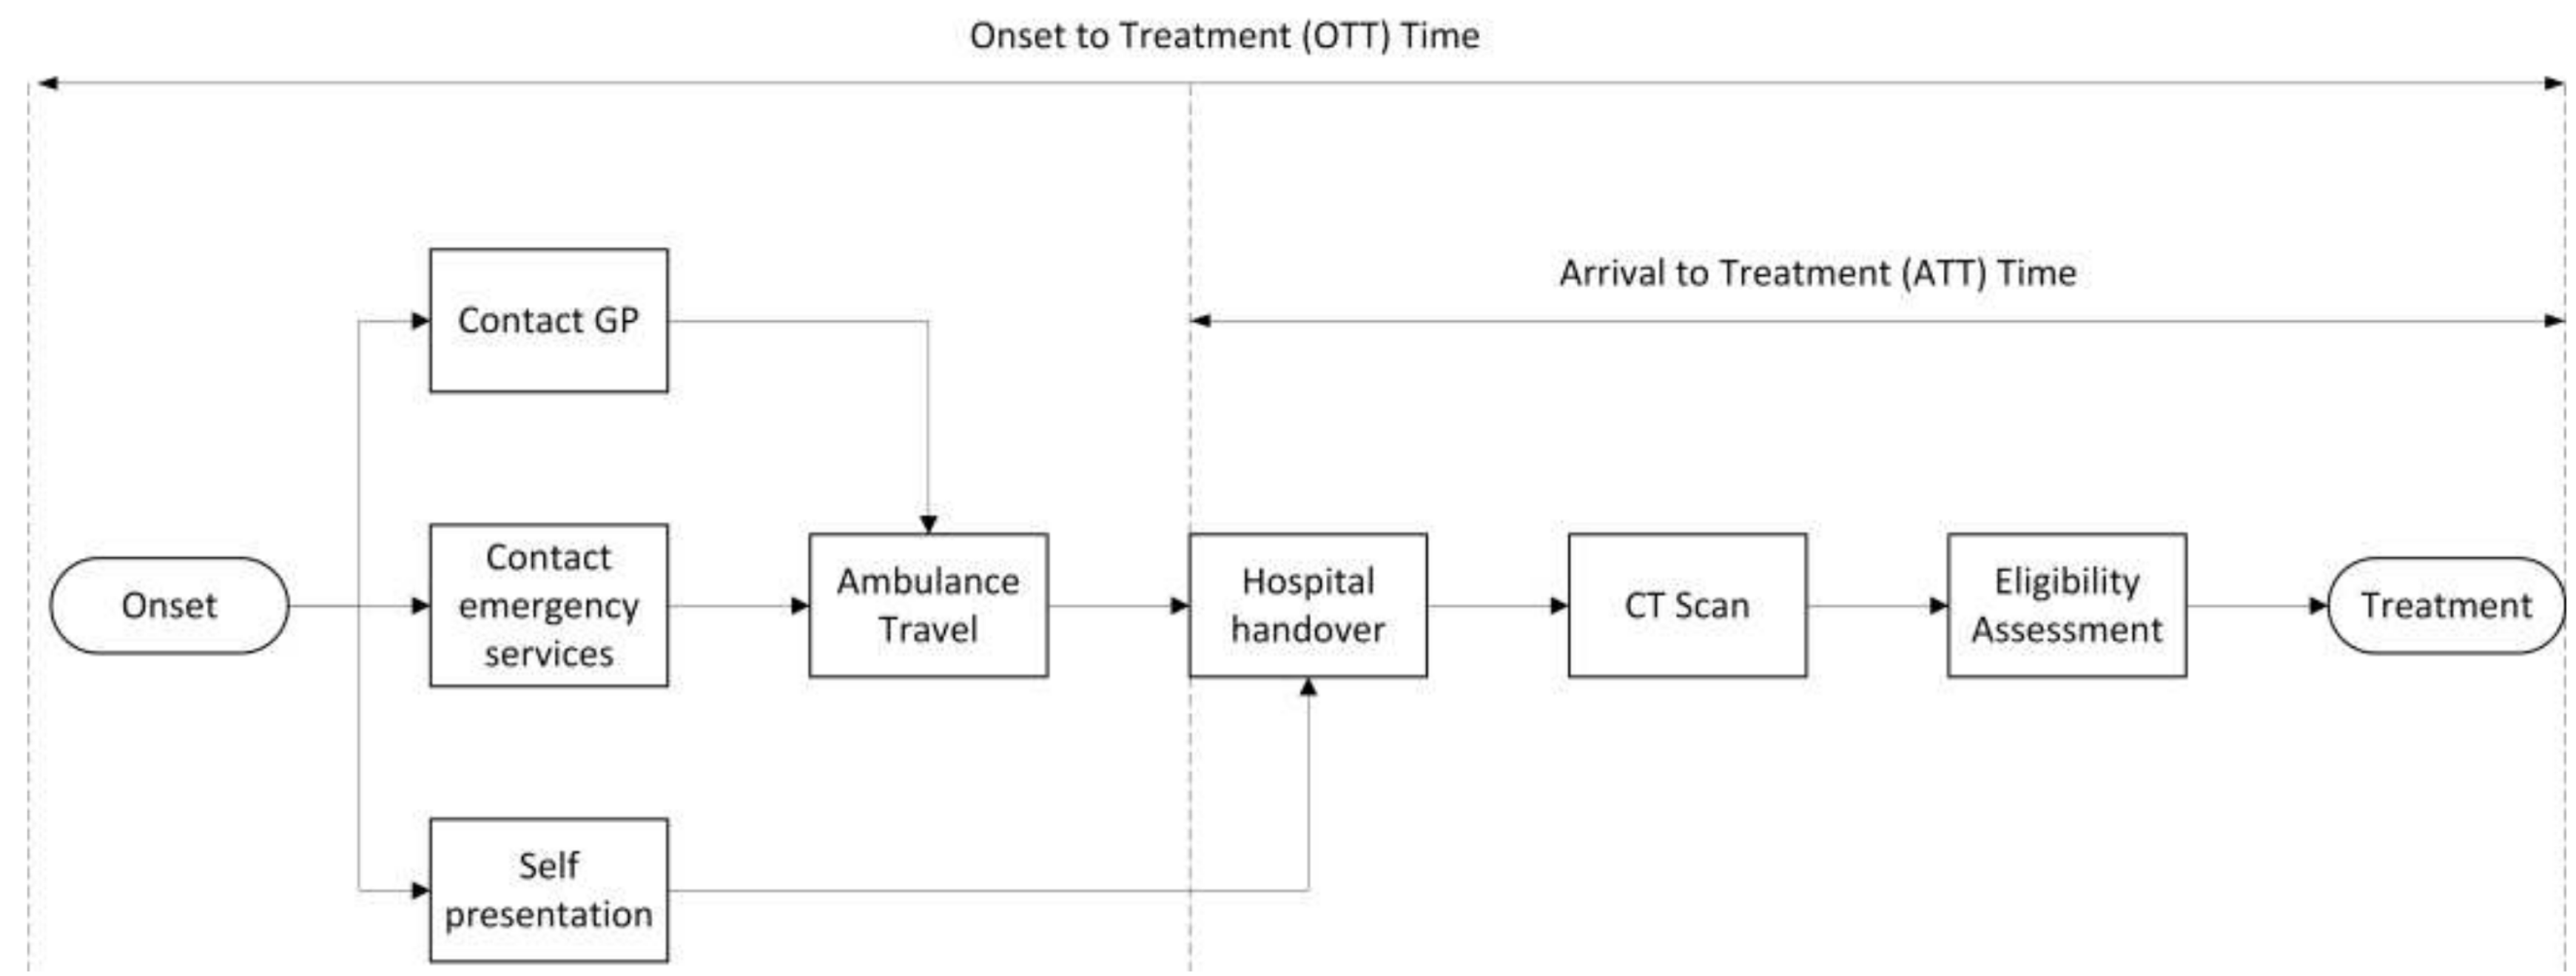
\includegraphics[width=0.75\linewidth]{images/monks_hyperacute_pathway.png}
    \caption{Modelling stroke care pathway to reperfusion treatment}
    \label{fig:monks_hyperacute_pathway}
\end{figure}

\begin{figure}
    \centering
    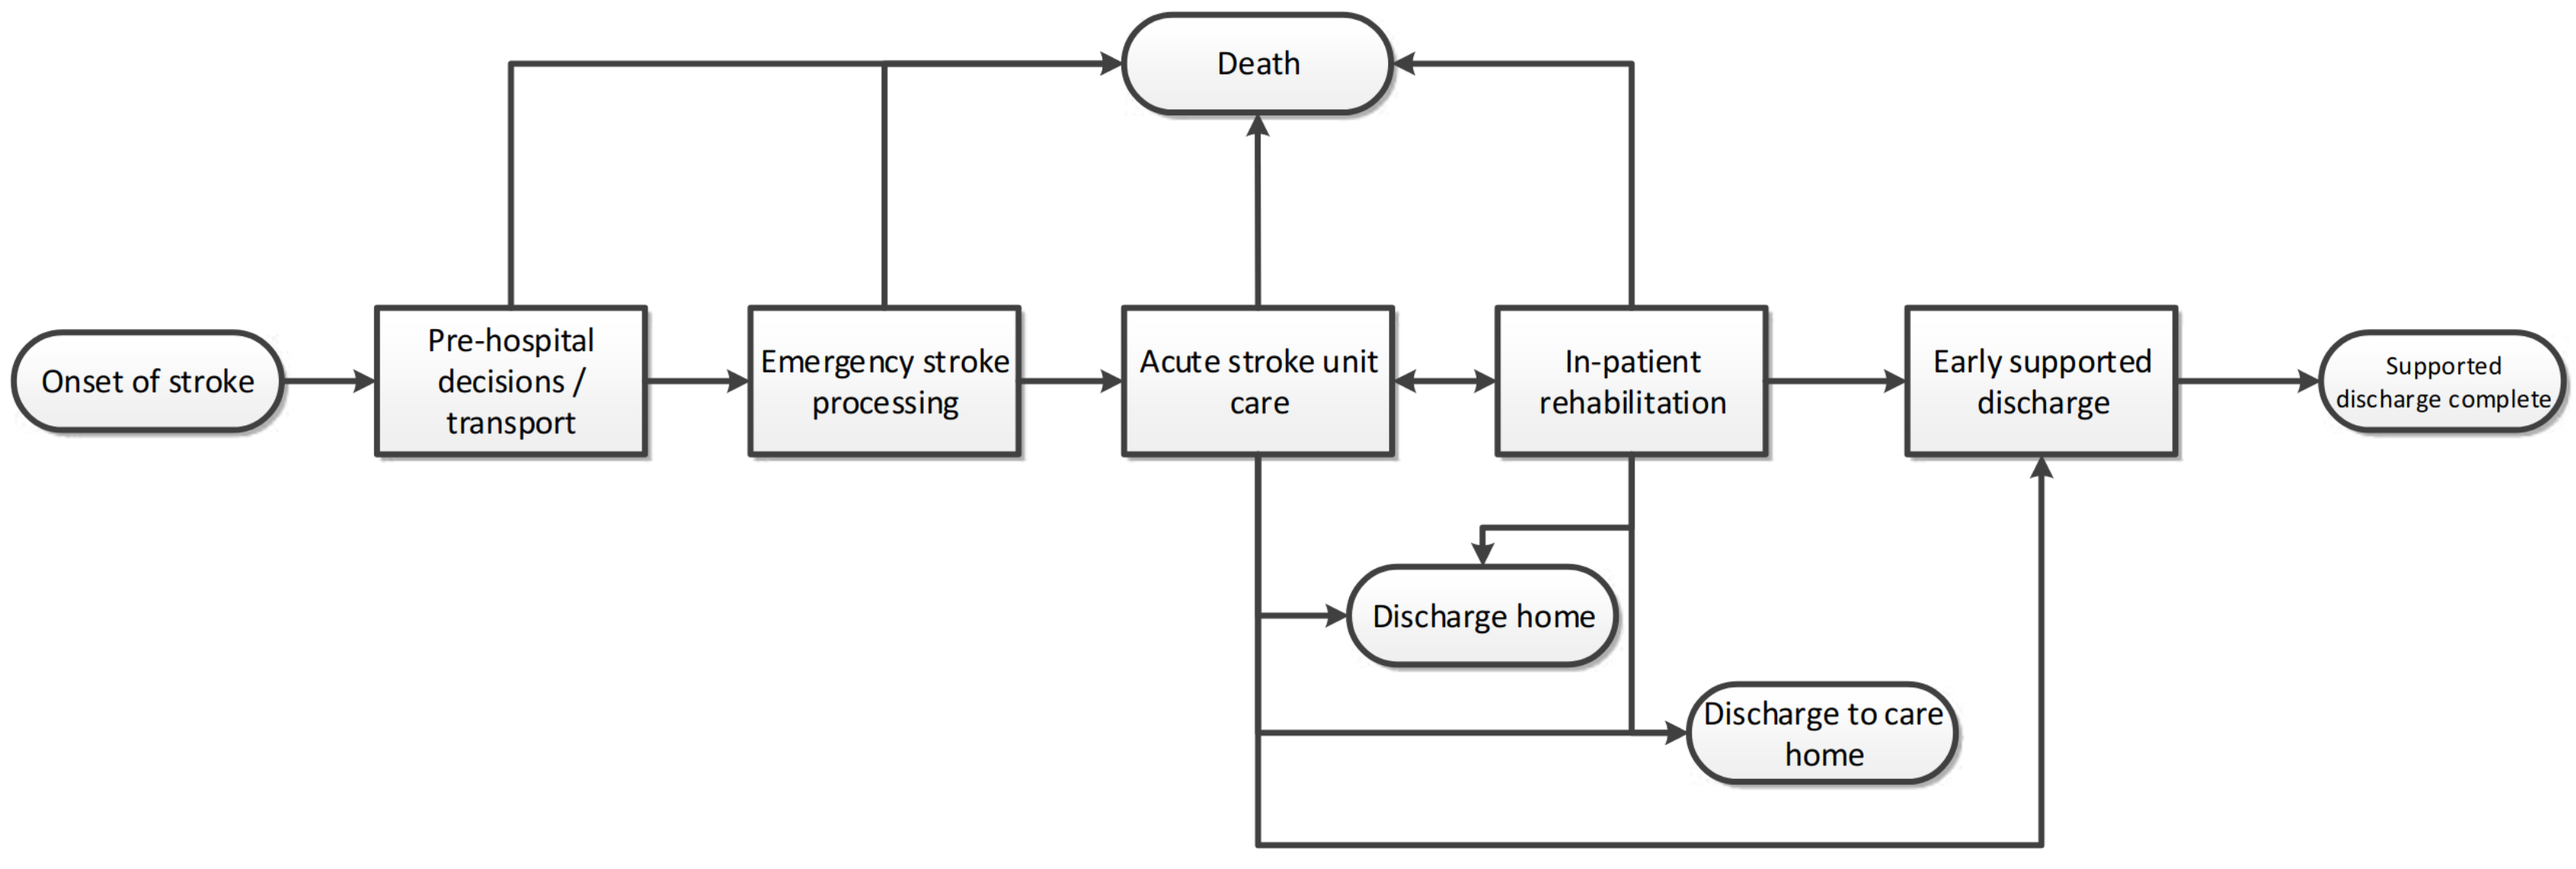
\includegraphics[width=0.75\linewidth]{images/monks_pathway.png}
    \caption{Modelling stroke care pathway to discharge}
    \label{fig:monks_pathway}
\end{figure}


